\section{One likelihood, three predictors}
\label{sec:framework}

The conceptual spine of \pkg{amore} is a single front-end, \texttt{rem()},
that fits a relational event model from already preprocessed case--control
data and dispatches to one of three estimation backends. The unifying claim
is deliberately precise. Two of the backends---the linear conditional logit
(\texttt{clogit}) and the neural multilayer perceptron (\texttt{nn})---maximize
the \emph{same} risk-set softmax conditional-logistic partial likelihood; they
differ only in how the per-candidate intensity is parameterized (a linear
predictor versus a learned nonlinear score). The third backend (\texttt{gam})
does \emph{not} share that likelihood: it fits the algebraically related
\emph{degenerate}, case-1-control binomial logistic regression of
\citet{boschi2025rhem}, in which the response is a constant and the linear
predictor is built from event-minus-control differences. This distinction is
load-bearing throughout the paper and we never collapse it: \texttt{clogit} and
\texttt{nn} are two parameterizations of one partial likelihood, while
\texttt{gam} is an algebraically related but distinct estimating equation that
buys smooth, time-varying, and random effects through \pkg{mgcv}.

\subsection{Formula syntax}
\label{sec:framework-formula}

The right-hand side of the model formula lists covariates. A bare name requests
a \textbf{linear} effect, available under all three backends. Three wrapper
functions request \emph{smooth} effects and are accepted only by the
\texttt{gam} backend:
\begin{itemize}
  \item \texttt{tv(x)} --- a time-varying linear effect, expanded to
    \texttt{s(time, by = d\_x)};
  \item \texttt{nl(x)} --- a non-linear effect, expanded to
    \texttt{s(cbind(x\_ev, x\_nv), by = c(1, -1))};
  \item \texttt{tvnl(x)} --- a time-varying non-linear effect, expanded to a
    tensor-product smooth \texttt{te(time, x, by = ...)}.
\end{itemize}
A fourth wrapper, \texttt{re(x)}, requests a \textbf{random effect} of a
grouping factor (for instance the sender). It is realized through a matched
factor-matrix construction that mirrors the case--control geometry: an
$n \times 2$ factor matrix holds the grouping level of the event in the first
column and of the matched control in the second, and is passed as
\texttt{s(cbind(x\_ev, x\_nv), by = cbind(1, -1), bs = "re")}. The
\texttt{by = cbind(1, -1)} contrast makes the term contribute
$f(\text{event level}) - f(\text{control level})$, so the random effect is
identified precisely when the event and its matched control differ on the
grouping variable (following the species-invasiveness term of the
introduction-to-REM tutorial). When the matched \texttt{x\_ev}/\texttt{x\_nv}
columns are absent, the construction falls back to a single column.

Column resolution is uniform across terms. For a linear covariate \texttt{x},
\texttt{rem()} takes the event-minus-control difference from column \texttt{x}
if present, else from \texttt{d\_x}, else from \texttt{x\_ev - x\_nv};
non-linear terms prefer \pkg{eventnet}'s spline-transformed
\texttt{transform\_x\_ev}/\texttt{transform\_x\_nv} columns when available. For
the \texttt{gam} backend the left-hand side of the formula is ignored (the
response is the constant case indicator); for \texttt{clogit} and \texttt{nn}
the left-hand side names the 0/1 event-indicator column (e.g.\
\code{event \textasciitilde{} x}), unless the indicator column is supplied
explicitly through the \texttt{case} argument.

\subsection{The \texttt{clogit} backend: linear conditional logit}
\label{sec:framework-clogit}

The \texttt{clogit} backend fits a conditional logistic regression on a
case-$k$-control design via \code{survival::clogit()}, restricted to linear
terms. Each observed event is grouped with its sampled non-events into a
stratum; the strata are taken from the \texttt{stratum} column, or derived as
\texttt{cumsum(case == 1)} when \texttt{stratum} is \texttt{NULL} (the blocked
``case-then-controls'' layout produced by \pkg{eventnet} and by the package's
own simulator). Writing $\eta_i = x_i^{\top}\beta$ for the linear predictor of
candidate $i$ and $\mathcal{R}_s$ for the risk set of stratum $s$ whose observed
event is $e(s)$, the conditional partial likelihood is
\begin{equation}
  \label{eq:cl-partial-likelihood}
  \mathrm{PL}(\beta)
  = \prod_{s} \frac{\exp\!\big(\eta_{e(s)}\big)}
                   {\sum_{i \in \mathcal{R}_s} \exp(\eta_i)},
\end{equation}
the familiar risk-set softmax of \citet{butts2008}, reduced to a sampled
case--control form following \citet{lerner2020}. This is the canonical
relational-event partial likelihood and the reference estimand against which
the \texttt{nn} backend is defined.

\subsection{The \texttt{gam} backend: degenerate logistic with smooth effects}
\label{sec:framework-gam}

The \texttt{gam} backend targets the \emph{degenerate} case-1-control logistic
regression of \citet{boschi2025rhem}. \texttt{rem()} assembles a response of
constant ones together with an internal $\pm 1$ contrast matrix, so that each
smooth or linear term enters as an event-minus-control difference, and passes
the result to \code{mgcv::gam()} with a binomial family and a no-intercept
formula (\code{one \textasciitilde{} -1 + ...}). This is the mechanism that
realizes the \texttt{tv}/\texttt{nl}/\texttt{tvnl}/\texttt{re} wrappers of
Section~\ref{sec:framework-formula}. The \texttt{gam\_method} argument controls
\pkg{mgcv}'s smoothness selection: it defaults to \texttt{NULL}, which lets
\pkg{mgcv} use its own default (\texttt{"GCV.Cp"}) and reproduces the
introduction-to-REM tutorial parameterization, and may be set to \texttt{"REML"}
for the REML fit used in some of the source papers. Because \pkg{mgcv} is a
\emph{Suggests} dependency, the backend raises an informative error at runtime
if the package is not installed.

We stress that this is a binomial GLM, not a stratified softmax fit. It
coincides numerically with a two-element conditional logit only under a single
matched control, a condition \texttt{rem()} does not enforce for the
\texttt{gam} path. Hence the careful wording: \texttt{gam} is
\emph{algebraically related} to Equation~\eqref{eq:cl-partial-likelihood}, not
an instance of it.

\subsection{The \texttt{nn} backend: a neural conditional logit}
\label{sec:framework-nn}

The \texttt{nn} backend replaces the linear predictor $\eta_i = x_i^{\top}\beta$
of Equation~\eqref{eq:cl-partial-likelihood} with a multilayer perceptron
$\eta_i = g_\theta(x_i)$ that scores each candidate jointly, while keeping the
loss \emph{exactly} the conditional partial likelihood. It is a pure-R
implementation with no extra dependencies, configured through
\code{nn\_control()} (hidden-layer sizes, ReLU or tanh activation, Adam learning
rate, $L_2$ weight decay, validation fraction, early-stopping patience, feature
standardization, and seed).

\paragraph{Forward pass.}
For a network with $L$ layers, hidden weight matrices $W^{(\ell)}$ and biases
$b^{(\ell)}$, the pre-activation and activation at layer $\ell$ are
\begin{equation}
  \label{eq:nn-forward}
  z^{(\ell)} = a^{(\ell-1)} W^{(\ell)} + b^{(\ell)},
  \qquad
  a^{(\ell)} = \phi\!\big(z^{(\ell)}\big) \ (\ell < L),
  \qquad
  a^{(0)} = x,
\end{equation}
with $\phi$ the ReLU or tanh activation and the final layer linear, so the
scalar score is $g_\theta(x_i) = z^{(L)}_i$. Weights use He initialization.

\paragraph{Loss.}
The loss is the per-stratum softmax negative log partial likelihood. With
$\mathcal{R}_s$ and $e(s)$ as before and $K$ the number of strata,
\begin{equation}
  \label{eq:nn-loss}
  \ell(\theta)
  = -\frac{1}{K}\sum_{s} \log
    \frac{\exp\!\big(g_\theta(x_{e(s)})\big)}
         {\sum_{i \in \mathcal{R}_s} \exp\!\big(g_\theta(x_i)\big)}.
\end{equation}
This is Equation~\eqref{eq:cl-partial-likelihood} with $g_\theta$ in place of
the linear predictor; with no hidden layers the backend reduces to a linear
conditional logit fit by gradient descent. A per-stratum max subtraction
stabilizes the softmax.

\paragraph{Gradient.}
The gradient of the loss with respect to the candidate scores has the
characteristic softmax-minus-indicator form
\begin{equation}
  \label{eq:nn-grad}
  \frac{\partial \ell}{\partial g_\theta(x_i)}
  = \frac{p_i - \mathbf{1}\{i = e(s_i)\}}{K},
  \qquad
  p_i = \frac{\exp\!\big(g_\theta(x_i)\big)}
             {\sum_{j \in \mathcal{R}_{s_i}} \exp\!\big(g_\theta(x_j)\big)},
\end{equation}
where $s_i$ is the stratum of candidate $i$ and $p_i$ its softmax probability.
This $(p - \mathbf{1}\{\text{event}\})/K$ vector is back-propagated through
Equation~\eqref{eq:nn-forward} by hand-derived analytic gradients, and the
parameters are updated by Adam with optional validation-based early stopping.
The gradients are verified against central finite differences, agreeing to
$\max|\text{analytic} - \text{numerical}| = 1.4\times 10^{-10}$ (experiment E6;
Section~\ref{sec:validation}).

\paragraph{What the backend reports, and what it does not.}
Because the score surface is learned rather than coefficient-indexed,
\code{coef()} returns \texttt{NULL} and there is no coefficient table, no
standard errors, and no uncertainty quantification. \code{summary()} instead
reports an in-sample top-1 concordance (the fraction of strata whose observed
event is scored highest) and, when a validation split is requested, a held-out
concordance. The backend accepts numeric covariates only and rejects factors
with an informative error, asking the user to encode them numerically first.
Training is pure R, full-batch by default but with optional mini-batch
stochastic gradient over strata (\code{batch\_strata}); it is intended for
accessibility, with the additive-spline architecture below the route to
larger problem sizes.

\paragraph{Interpretability via partial dependence.}
Although the network exposes no coefficients, \code{plot(fit, type = "pdp")}
recovers interpretable per-feature effects post hoc: for each feature it sweeps
a grid (two standard deviations either side of the mean) while holding the
others at their means, and plots the resulting partial score. This is how a
practitioner reads off the shape of a learned effect. Crucially, because the MLP
scores the full candidate vector jointly rather than additively, it can
represent cross-feature \emph{interactions} that the additive backends cannot.
On a planted multiplicative truth $\eta = 2.5\,x_1 x_2$, the \texttt{nn} backend
attains an in-sample concordance of $0.81$ against $0.52$ for the linear
\texttt{clogit}, which is stuck near chance; on a purely linear truth the two
tie at $0.78$, so the added flexibility carries no penalty when it is not needed
(experiment E6, Figure~\ref{fig:exp6-nn}). We frame this strictly as an
accessibility and engineering contribution. Flexible relational-event
modelling is not new: STREAM \citep{filippimazzola2024} fits additive
B-spline effects by minibatch stochastic gradient on the same case-control
logistic objective at the scale of $10^{8}$ events, and the neural
temporal-point-process literature---recurrent marked temporal point processes
\citep{du2016} and the neural Hawkes process \citep{mei2017}---predates this
package. \pkg{amore}'s contribution is a GPU-free, zero-extra-dependency,
numerically verified neural conditional logit reachable from a plain
\code{install.packages()}, not a claim of priority.

\paragraph{An additive-spline architecture.}\label{sec:framework-nn-additive}
The same loss and optimizer also serve a second, interpretable architecture:
\code{nn\_control(architecture = "additive\_spline")} expands each covariate
in a B-spline basis and fits a single linear layer over the concatenated
bases, so the score is the additive model $\eta = \sum_k f_k(x_k)$ trained by
(mini-batch) stochastic gradient on the exact risk-set softmax partial
likelihood. With one sampled control this is precisely the STREAM
construction that \citet{filippimazzola2024} used to fit smooth citation
effects on $10^{8}$ patent events --- the same estimand as a basis-expanded
conditional logit, optimized stochastically so that memory no longer scales
with the full design. The \code{batch\_strata} option takes one Adam step per
sampled chunk of strata, and the fitted per-feature curves are read directly
from \code{plot(type = "pdp")}. The package thus offers smooth additive
effects on \emph{both} case-control objectives: on the degenerate
case-1-control regression through \pkg{mgcv} (\code{method = "gam"}), and on
the exact softmax partial likelihood through stochastic gradient
(\code{method = "nn"}).

\begin{figure}[t]
  \centering
  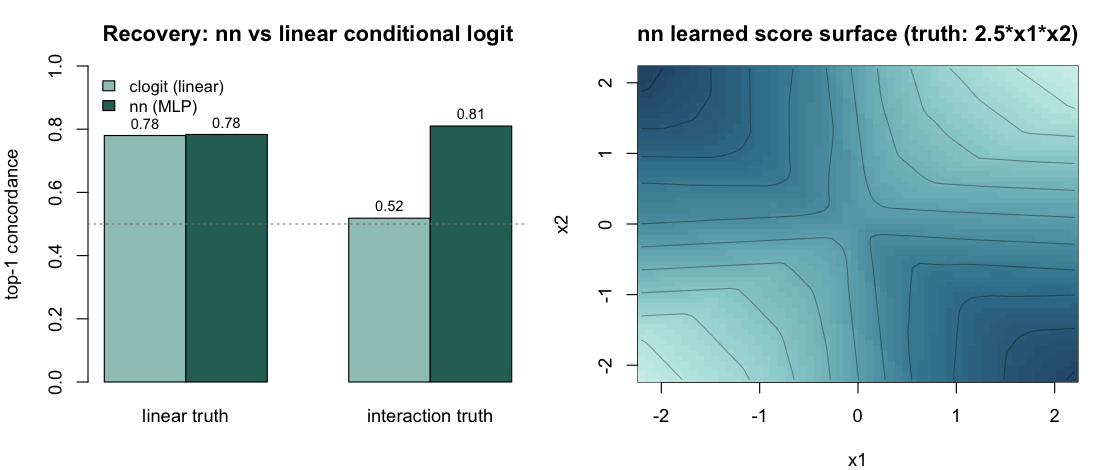
\includegraphics[width=0.9\linewidth]{figs/exp6-nn.png}
  \caption{Neural backend (experiment E6). Left: top-1 concordance of the
    \texttt{nn} MLP versus the linear \texttt{clogit} under a linear truth (tie
    at $0.78$) and a multiplicative interaction truth ($0.81$ vs $0.52$).
    Right: the learned score surface over $(x_1, x_2)$, recovering the
    opposite-sign corners of the interaction. Concordance figures are in-sample.}
  \label{fig:exp6-nn}
\end{figure}

\subsection{One front-end, one object contract}
\label{sec:framework-contract}

All three backends return an object of class \texttt{rem}: a list holding the
fitted model in \texttt{\$fit}, the chosen \texttt{method}, the original
\texttt{formula}, the parsed terms, and the number of observations. The shared
S3 methods (\code{print()}, \code{summary()}, \code{coef()}, \code{plot()},
\code{logLik()}, \code{predict()}) delegate to \texttt{\$fit}, so downstream code
is written once against the \texttt{rem} contract regardless of backend; the
\texttt{nn} fit carries its own inner methods (for instance the
partial-dependence plot) to which the outer \texttt{rem} methods forward. A
minimal end-to-end call looks as follows.

\begin{verbatim}
set.seed(1)
## long case-control layout (one row per candidate): clogit / nn
d <- simulate_relational_events(
  n_events = 300,
  senders = paste0("a", 1:12), receivers = paste0("a", 1:12),
  n_controls = 1, endogenous_stats = "reciprocity_count",
  endogenous_effects = c(reciprocity_count = 0.6))

## wide case-1-control layout (one row per event): gam
w <- simulate_relational_events(
  n_events = 300,
  senders = paste0("a", 1:12), receivers = paste0("a", 1:12),
  n_controls = 1, endogenous_stats = "reciprocity_count",
  endogenous_effects = c(reciprocity_count = 0.6), wide = TRUE)

## linear conditional logit
fit_cl <- rem(event ~ reciprocity_count, data = d, method = "clogit")

## smooth / time-varying via mgcv
fit_gam <- rem(~ tv(reciprocity_count), data = w, method = "gam", time = "time")

## neural conditional logit
fit_nn <- rem(event ~ reciprocity_count, data = d, method = "nn",
              nn = nn_control(hidden = c(16, 8), seed = 1))
summary(fit_nn)
plot(fit_nn$fit, type = "pdp")
\end{verbatim}

Each backend consumes the case--control data in the layout it expects:
\texttt{gam} the wide, one-row-per-event frame (\texttt{wide = TRUE}, carrying
event-minus-control difference columns), and \texttt{clogit} and \texttt{nn} the
long, one-row-per-candidate frame (carrying a 0/1 event indicator and a
stratum). Both layouts are produced by the same source---the package's own
simulator, or \pkg{eventnet}---so the user chooses linear, smooth, or neural by
switching a single \texttt{method} argument, and reads the result through one
object interface.
